\chapter{Physiologische Grundlagen}\label{chap:Physiologische Grundlagen}

%Bei den physiologischen Grundlagen könnte das in Richtung Algorithmendesign und Notwendigkeit der Interpretierbarkeit automatisierter Klassifikationsergebnisse gehen, die jeweils das Verständnis der physiologischen Grundlagen und der Pathophysiologie bei VHF voraussetzen.

Um einen Algorithmus zur automatisierten Detektion von \gls{VHF} im \gls{EKG} zu designen, sowie die durch den Algorithmus erstellten Klassifikationsergebnisse zu interpretieren, wird das Verständnis von physiologischen Grundlagen der Erregungsabläufe im Herzen sowie der Pathophysiologie bei \gls{VHF} benötigt.
Aus diesem Grund wird in diesem Kapitel zuerst in \hyperref[sec:Erregungsleitsystem]{Abschnitt 2.1} das Erregungsleitsystem des gesunden Herzens erläutert, sowie in dem darauffolgenden \hyperref[sec:myozyten]{Abschnitt 2.2} die Funktionsweise von Kardiomyozyten. Die Entstehung von \gls{VHF} wird in \hyperref[sec:Vorhofflimmern]{Abschnitt 2.3} erklärt. Anschließend wird in \hyperref[sec:DiagVorhofflimmern]{Abschnitt 2.4} auf die signaltechnische Erfassung, sowie die Diagnostik von \gls{VHF} mittels \gls{EKG} eingegangen.


\section{Erregungsleitsystem des Herzens}\label{sec:Erregungsleitsystem}

Das Herz dient der Blutzirkulation im Körper und stößt im Ruhezustand durchschnittlich mit einer Frequenz von 70 Schlägen/min sauerstoffreiches Blut in den Körper- und sauerstoffarmes Blut in den Lungenkreislauf aus \cite{gekle_taschenlehrbuch_2015}. Es teilt sich durch die Herzscheidewand (Septum) in zwei Hälften, welche jeweils einen Vorhof (Atrium) und eine Kammer (Ventrikel) besitzen. Zwischen dem rechten Vorhof und der rechten Kammer befindet sich die Trikuspidalklappe, zwischem dem linken Vorhof und der linken Kammer die Bikuspidalklappe (Mitralklappe). In den vom Herzen wegführenden Gefäßen (der Aorta und der Lungenschlagader Truncus pulmonalis) befinden sich  Taschenklappen.  \cite{zilles_anatomie_2010} 

Die Herzmuskulatur (Myokard) besitzt die Fähigkeit, ohne externe Nervenimpulse Erregungen auszubilden und zu kontrahieren. Die Herzmuskelzellen (Kardiomyozyten) in verschiedenen Bereichen des Herzens besitzen diese Fähigkeit je nach Zelltyp in unterschiedlich starken Ausprägungen. Spezialisierte Myozyten im Herzen bilden das Erregungsleitungssystem, welches für eine koordinierte Erregungsbildung und -weiterleitung zuständig ist. Dies ist in \hyperref[fig:HerzPhys]{Abb.~2.1} schematisch dargestellt. Als Arbeitsmyokard werden spezialisierte Myozyten bezeichnet, welche zur Kontraktion fähig sind \cite{gertsch_ekg_2007}. Der Sinusknoten, welcher im rechten Vorhof in Höhe der Einmündung der oberen Hohlvene liegt, besteht aus Myozyten zur Erregungsbildung. Er dient als primäres Erregungszentrum des Myokards und bildet 60-80 Erregungen pro Minute aus. Die vom Sinusknoten ausgehenden Reize breiten sich in das Arbeitsmyokard der Vorhöfe aus, welches nach ca. 90 ms vollständig erregt ist und kontrahiert \cite{gekle_taschenlehrbuch_2015}. \cite{zilles_anatomie_2010}

Das Herzskelett trennt die Vorhöfe vollständig von den Kammern, sodass auch Erregungen nicht von den Vorhofmyozyten auf die Kammermyozyten übergehen können. Lediglich der \gls{AV-Knoten}, welcher am Übergang zwischen Vorhofseptum und Ventrikelseptum lokalisiert ist, ist in der Lage, Erregungen von den Vorhöfen in die Kammern weiterzuleiten \cite{zilles_anatomie_2010}. Die Myozyten des \gls{AV-Knoten}s besitzen mit 0,05 m/s eine geringere Reizweiterleitungsgeschwindigkeit als Vorhofmyozyten, bei welchen sie bei 0,5 m/s liegt. Durch die verzögerte Reizweiterleitung in die Kammern ist die Kontraktion der Vorhöfe beendet, bevor die Kammern kontrahieren. Auf diese Weise wird sichergestellt, dass die Kammern vor der Kontraktion ausreichend mit Blut gefüllt sind. Die verzögerte Reizweiterleitung sorgt bei pathologisch hohen Erregungsfrequenzen im Vorhof dafür, dass nicht jede Erregung in das Kammermyokard weitergeleitet wird, sodass sich die Kammern trotz dessen vor der Kontraktion ausreichend füllen können.  Der \gls{AV-Knoten} verfügt wie der Sinusknoten über die Fähigkeit, autonom Erregungen zu erzeugen. Kommt es durch pathophysiologische Bedingungen zu einem Ausfall des Sinusknotens, kann der \gls{AV-Knoten} mit einer Frequenz von 40-50 Erregungen pro Minute als sekundärer Schrittmacher dienen. \cite{gekle_taschenlehrbuch_2015} 

\begin{figure}[!ht]%
\centering
	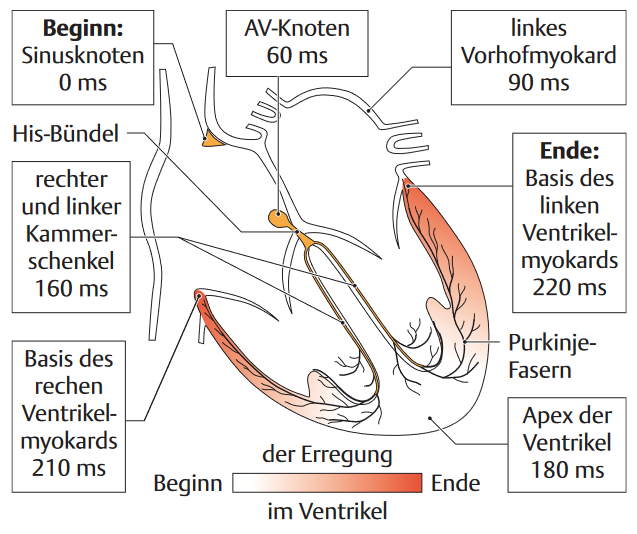
\includegraphics[width=0.80\textwidth]{./Bilder/HerzPhys.png}
\caption[Darstellung des Erregungsleitsystems des Herzens]{Darstellung des Erregungsleitsystems des Herzens. Zu sehen ist die Erregungsausbreitung vom Beginn im Sinusknoten bis zum Ende im Myokard des linken Vorhofes. Zusätzlich angegeben ist die Dauer der Erregungsausbreitung. Entnommen aus \cite{gekle_taschenlehrbuch_2015}.} 
\label{fig:HerzPhys}
\end{figure}  

Vom \gls{AV-Knoten} aus wird die Erregung über das His-Bündel geleitet, über den linken und rechten Tawara-Schenkel am Kammerseptum entlang und in die Purkinje-Fasern hinein. Dieser Teil des Erregungsleitungssystems ist von den Kammermyozyten elektrisch isoliert. Erst die Purkinje-Fasern verzweigen sich ins Kammermyokard und übertragen den Reiz an die Kammermyozyten. Die Zeitspanne von Erregungsbildung im Sinusknoten bis zur vollständigen Erregung der Kammermyozyten beträgt ca. 220 ms. Im Anschluss an die Kammererregung erfolgt die Kammerkontraktion.~\cite{gekle_taschenlehrbuch_2015} 

\section{Funktionsweise der Kardiomyozyten}\label{sec:myozyten}

Wie bereits im vorherigen \hyperref[sec:Erregungsleitsystem]{Abschnitt 2.1} erwähnt, gibt es verschiedene Typen von Kardiomyozyten, welche unterschiedliche Funktionen aufweisen: Erregungsbildung (Sinusknoten), Erregungsweiterleitung (\gls{AV-Knoten} und Purkinjefasern) und Kontraktion (Arbeitsmyokard der Vorhöfe und Kammern). Die Myozyten zur Erregungsbildung und -weiterleitung besitzen außerdem die Fähigkeit, autonom einen Reiz auszulösen, die Myozyten des Arbeitsmyokards nicht. Die Ursache hierfür liegt in den unterschiedlichen Aktionspotentialen der Zelltypen begründet. Ein Aktionspotential ist eine starke Änderung des Membranpotentials einer Zelle und dient der Informationsübertragung. Der Verlauf der Aktionspotentiale (siehe \hyperref[fig:Aktionspotential]{Abb.~2.2}) wird in die Phasen 0 bis 4 eingeteilt, welche im Folgenden näher erläutert werden. \cite{gekle_taschenlehrbuch_2015}

Eine Zelle des Arbeitsmyokards ist in Ruhe bei -90 mV polarisiert (Ruhemembranpotential), dies wird als Phase 4 bezeichnet. Erreicht die Zelle ein elektrischer Reiz, depolarisiert sie auf 0 mV, wobei Natrium-Ionen durch spezifische Kanäle in die Zelle hinein fließen. Dies ist Phase 0 und der Beginn des Aktionspotentials. Während der Depolarisation kommt es zu einem Overshoot, bei welchem die Zelle kurzzeitig bei 20 mV polarisiert ist (Phase 1). \cite{gertsch_ekg_2007}

Auf den Overshoot folgt eine kurze Repolarisation mit anschließendem Plateau im Aktionspotential (Phase 2). Die initiale Repolarisation kommt durch das Fließen von Kalium-Ionen aus der Zelle heraus zustande. Im Laufe dessen öffnen sich Calcium-Ionen-Kanäle, durch die Calcium-Ionen in die Zelle hinein fließen und den Auswärtsstrom der Kalium-Ionen ausgleichen, wodurch das Plateau entsteht. Der Einwärtsstrom der Calcium-Ionen leitet die Kontraktion des Myozyts ein. \cite{gekle_taschenlehrbuch_2015}

In Phase 3 repolarisiert die Zelle durch einen Kalium-Ionen Auswärtsstrom  bis sie sich wieder im Ruhemembranpotential, also in Phase 4, befindet. Die Zelle verbleibt in Phase 4, bis ein erneuter Reiz zur Depolarisation führt. Aufrechterhalten wird das Ruhemembranpotential durch einen kontinuierlichen Austausch von Natrium- und Kalium-Ionen zwischen Intra- und Extrazellulärraum. \cite{gertsch_ekg_2007} 

Übertragen wird ein Reiz von benachbarten Myozyten über sogenannte Gap Junctions, die aus einer Ansammlung unspezifischer Ionenkanäle bestehen, die Connexone genannt werden~\cite{gekle_taschenlehrbuch_2015}.

\begin{figure}[!ht]%
\centering
	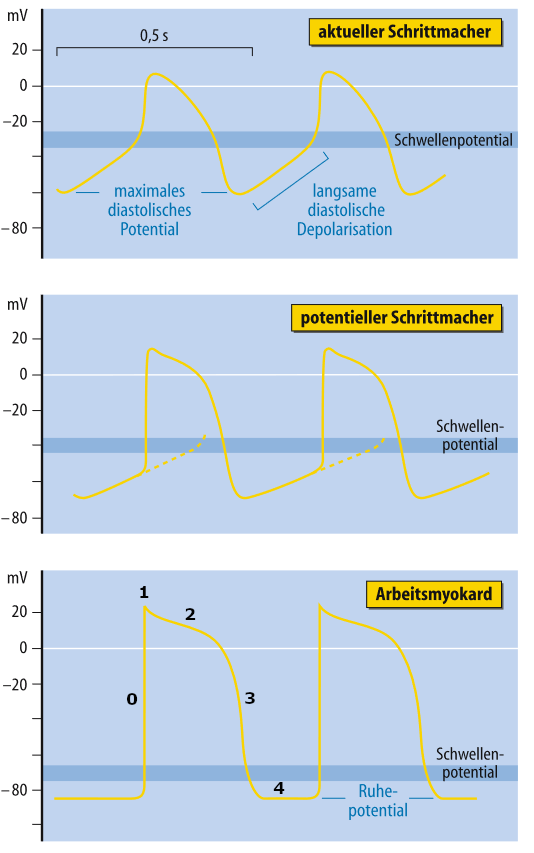
\includegraphics[width=0.80\textwidth]{./Bilder/Aktionspotentiale.png}
\caption[Darstellung von Aktionspotentialen verschiedener Zellen]{Darstellung der Aktionspotentiale einer Sinusknotenzelle (oben), einer Erregungsleitungszelle (mitte) und einer Zelle des Arbeitsmyokards (unten), abgeändert entnommen aus \cite{schmidt_physiologie_2005}. Die Phasen 0 bis 4 des Aktionspotentialverlaufs sind eingetragen.} 
\label{fig:Aktionspotential}
\end{figure}  

Im Gegensatz zu einem Myozyt des Arbeitsmyokards können Sinusknotenmyozyten und Myozyten des Reizleitungsgewebes autonom eine Erregung generieren. Diese Fähigkeit besitzen sie, da sie kein stabiles Ruhemembranpotential haben, sondern in Phase 4 langsam depolarisieren (Spontandepolarisation \cite{schmidt_physiologie_2005}). Diese Depolarisation wird hauptsächlich durch HCN-Kanäle (hyperpolarization activated cyclic nucleotide gated channels) verursacht, durch welche Ionen in die Zelle hineinfließen. Das maximale negative Potential eines Sinusknoten- oder Reizleitungsmyozyts liegt bei -60 mV. Erreicht die Zelle bis zu einem Schwellwert von ca. -40 mV kein Reiz, depolarisiert sie autonom \cite{schmidt_physiologie_2005}. Sinusknoten- und \gls{AV-Knoten}-Myozyten besitzen keine Phase 1 und 2 im Aktionspotential. Bei Myozyten des Sinusknotens wird dieser Schwellwert schneller erreicht, als bei Myozyten des Reizleitungsgewebes, weshalb der Sinusknoten als der primäre Schrittmacher fungiert. Fällt der Sinusknoten aus, kann der \gls{AV-Knoten} als sekundärer Schrittmacher dienen, fällt auch dieser aus, können Teile des Erregungsleitsystems der Ventrikel als tertiärer Schrittmacher einspringen. \cite{gekle_taschenlehrbuch_2015}

Kardiomyozyten sind für einige Zeit nach Beginn der Phase 0 nicht erregbar. Diese Zeit wird als absolute Refraktärphase bezeichnet. Erst wenn das Aktionspotential in Phase 3 wieder bei ca. -40 mV liegt, ist die Zelle wieder durch Reize erregbar. Dies ist die relative Refraktärphase. Um die Zelle in der relativen Refraktärphase zu erregen, ist jedoch ein erheblich stärkerer Reiz notwendig als vom Ruhemembranpotential aus. Da die Refraktärphase länger ist als die Dauer, die zur Depolarisation benötigt wird, wird durch sie eine rückläufige Erregungsausbreitung im Herzen verhindert. \cite{gekle_taschenlehrbuch_2015}


Das Herz muss in der Lage sein, sich dem Bedürfnis des Körpers nach einer erhöhten Sauerstoffversorgung, bspw. beim Sport, anzupassen. Dies wird unter anderem durch eine Erhöhung der Herzfrequenz und der Arbeitslast des Herzens erreicht. Dies ist möglich, da das Herz von Nerven des autonomen Nervensystems innerviert ist. Sympathikus und Vagusnerv haben Einfluss auf die Geschwindigkeit der Spontandepolarisation der Sinusknotenzellen, wodurch eine Frequenzsteigerung (positive Chronotropie) durch Stimulation durch den Sympathikus oder Frequenzsenkung (negative Chronotropie) durch Aktivität des Vagusnervs erzielt wird. Ebenso wird eine Erhöhung der Reizleitungsgeschwindigkeit im \gls{AV-Knoten} (positive Dromotropie) durch Stimulation durch den Sympathikus bzw. Verringerung der Reizleitungsgeschwindigkeit (negative Dromotropie) durch Stimulation durch den Vagusnerv  erzielt. \cite{schmidt_physiologie_2005}

%TODO Refraktärphase mehr? re-entry und vulnerable phase beschreiben

\section{Pathophysiologie von Vorhofflimmern}\label{sec:Vorhofflimmern}

\gls{VHF} ist eine Herzrhythmusstörung, bei der die Vorhoferregung gestört ist und die Vorhöfe somit schnell und unregelmäßig kontrahieren. Durch diese unkoordinierten Vorhofaktionen wird unter Belastung oder bei fortgeschrittenem \gls{VHF} die Füllung der Ventrikel erheblich beeinträchtigt, sodass nicht bei jeder Kammerkontraktion genug Blut ausgestoßen wird. \cite{rizwan_review_2021}

\gls{VHF} wird unterteilt in paroxysmales, persistierendes und permanentes \gls{VHF}, wobei diese Charakterisierung die Dauer der \gls{VHF}-Episode beschreibt. Als paroxysmal wird \gls{VHF} bezeichnet, wenn es unter einer Woche andauert und eigenständig endet (spontane Konversion \cite{gertsch_ekg_2007}). Dauert das \gls{VHF} länger als 7 Tage an, ist eine Kardioversion nötig und das \gls{VHF} wird als persistierend bezeichnet. Persistierendes \gls{VHF} kann in permantentes \gls{VHF} übergehen, wenn die Kardioversion nicht erfolgreich (oder gar nicht) durchgeführt wurde. Im Falle des permanenten \gls{VHF} ist dieses dauerhaft bestehend. \cite{erdmann_klinische_2011} 

Die Entstehung von \gls{VHF} ist ein Zusammenspiel aus Auslösern und Aufrechterhaltungsmechanismus (siehe \hyperref[fig:VHFschematic]{Abb.~2.3}) durch verändertes Gewebe im Vorhof. Die Veränderung des Gewebes zeichnet sich durch Umbau der elektrischen Reizleitungsbahnen sowie strukturelle Veränderungen des Vorhofgewebes aus (auch als Remodelling bezeichnet). \cite{wijesurendra_mechanisms_2019} 

\begin{figure}[!ht]%
\centering
	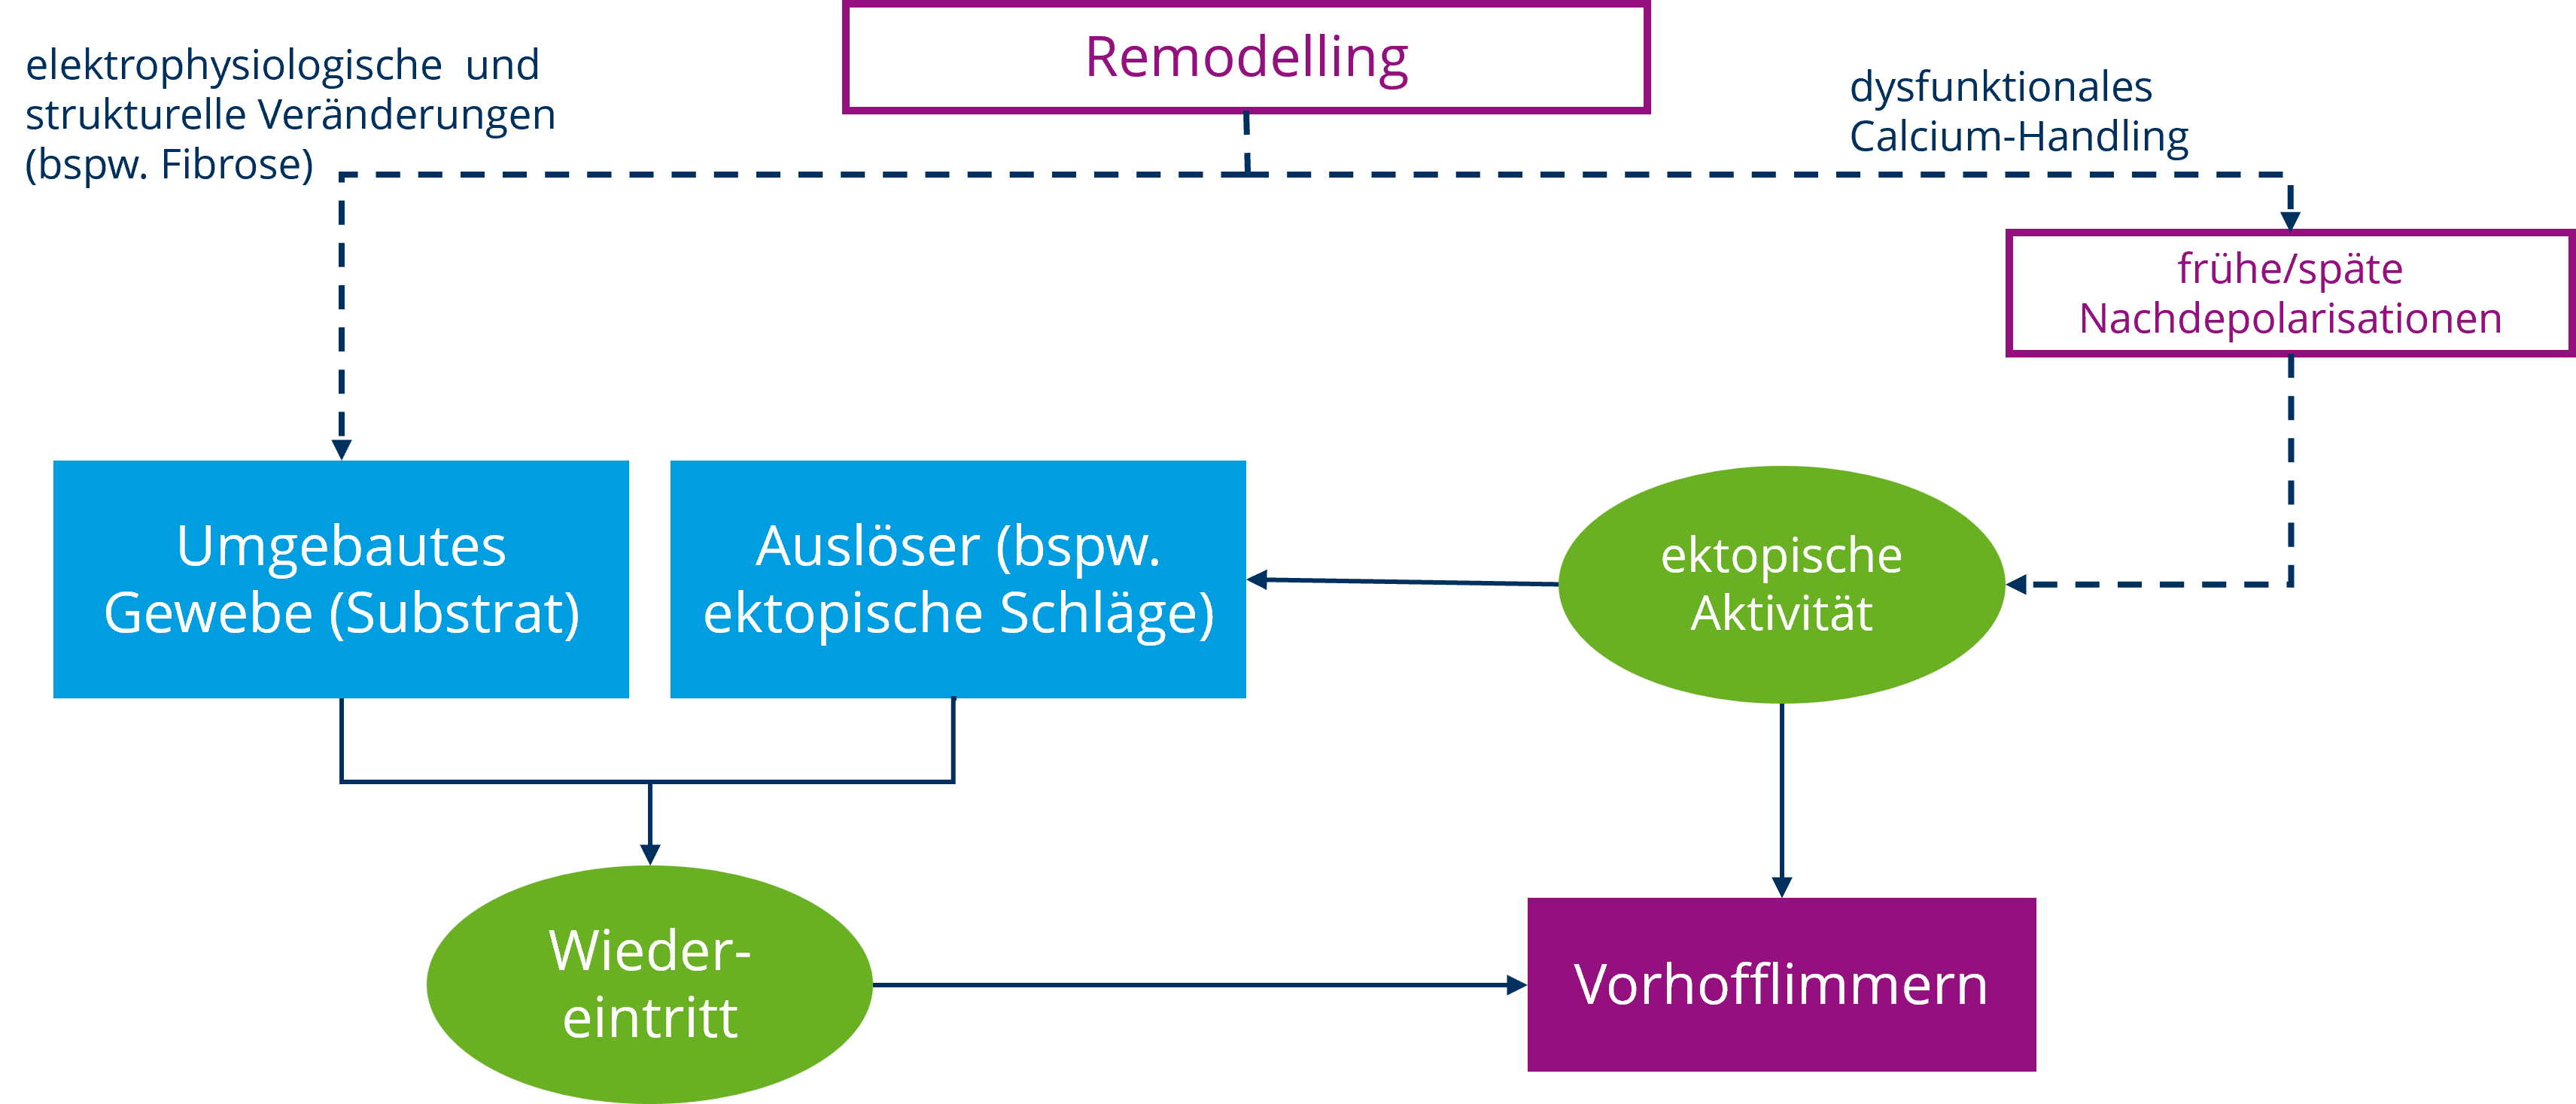
\includegraphics[width=1.0\textwidth]{./Bilder/VHFschematic_new.png}
\caption[Diagramm zur Pathophysiologie von VHF]{Schematische Darstellung von Mechanismen, die zu Vorhofflimmern führen. Eine dysfunktionales Calcium-Handling führt zu frühen oder verspäteten Nachdepolarisationen, welche ektopische Aktivität auslösen. Findet die ektopische Aktivität in hoher Frequenz statt, kann sie Vorhofflimmern aufrecht erhalten. Sie kann auch eine kreisende Erregung verursachen, die Vorhofflimmern aufrecht erhält. Auch ein struktureller und elektrophysiologischer Umbau des Vorhofmyokards kann zu kreisenden Erregungen und damit zu Vorhofflimmern führen. Entommen und übersetzt aus \cite{wijesurendra_mechanisms_2019}.} 
\label{fig:VHFschematic}
\end{figure} 

\subsection{Auslöser von Vorhofflimmern} \label{sec:auslöser}

Paroxysmale \gls{VHF}-Episoden werden durch spontane Depolarisationen von Gewebe mit erhöhter Automatik in oder außerhalb der Vorhöfe (bspw. in der Lungenvene) verursacht. Myozyten, die eine erhöhte Automatik aufweisen, haben ein weniger niedriges maximales negatives Potential, die spontane Phase-4-Depolarisation läuft schneller ab und ein niedrigeres Schwellenpotential ist vorhanden.
Nachdem ein Myozyt mit erhöhter Automatik einen Reiz generiert hat, kann es zu sogenannten frühen Nachdepolarisationen oder verzögerten Nachdepolarisationen kommen. Eine frühe Nachdepolarisation tritt während eines übermäßig verlängerten Aktionspotentials in Phase 3 auf, welches dafür sorgt, dass die deaktivierten Calcium-Kanäle sich erholen und erneut zu einem Calcium-Ionen-Fluss in den Myozyt hinein führen \cite{nattel_molecular_2020}. Eine verzögerte Nachdepolarisation tritt auf, nachdem ein Myozyt bereits zum Ruhemembranpotential zurückgekehrt ist. Sie wird verursacht durch einen Calcium-Überschuss innerhalb der Zelle, der durch Natrium-Calcium-Austauscher zu einem positiven Natrium-Ionen-Fluss in die Zelle hinein führt. Sind die Nachdepolarisationen stark genug, um das Schwellenpotential zu überschreiten, wird ein erneutes Aktionspotential ausgelöst. \cite{khan_identifying_2004}

Die ektopischen Depolarisationen zeichnen sich mit 350 bis 600 Reizen pro Minute durch eine höhere Frequenz als die des Sinusknotens aus \cite{sigg_cardiac_2010}. Hauptausgangspunkt der ektopischen Depolarisationen stellen in 94\% der Fälle die Pulmonalvenen dar \cite{haissaguerre_spontaneous_1998}. Dies liegt daran, dass das Gewebe der Pulmonalvenen andere elektrophysiologische Eigenschaften aufweist, als das Vorhofgewebe \cite{chen_initiation_1999}. Es konnten Myozyten in den Pulmonalvenen nachgewiesen werden, die eine besondere Leitfähigkeit aufweisen, bspw. Schrittmacherzellen und Purkinje-Zellen \cite{perez-lugones_evidence_2003}.
Neben den Pulmonalvenen kann \gls{VHF} auch durch anders verortete ektopische Depolarisationen ausgelöst werden, wie bspw. am Vorhofseptum oder an der posterioren Wand des linken Vorhofs  \cite{santangeli_techniques_2017}. 

Eine Unausgeglichenheit des autonomen Nervensystems kann als Auslöser der ektopischen Aktivität dienen. Hammer et al. \cite{hammer_cardiovascular_2023} zeigen, dass \gls{VHF}-Episoden eine erhöhte Aktivität des Sympathikus vorausgeht, gefolgt von einer erhöhten Aktivität des Vagusnervs.  Eine durch dysfunktionale Sympathikusaktivität erhöhte Ausschüttung von Calcium führt zu einer erhöhten Frequenz von Aktionspotentialen. Eine dysfunktionale Aktivität des Vagusnervs wiederum führt zu einer verkürzten Aktionspotentialdauer und Refraktärperiode. \cite{khan_heart_2019}

\subsection{Aufrechterhaltung von Vorhofflimmern}

\gls{VHF} kann durch die im \hyperref[sec:auslöser]{vorherigen Abschnitt} erwähnten ektopischen Aktivitäten aufrechterhalten werden, wenn diese schnell und andauernd stattfinden. Mit länger anhaltendem \gls{VHF} kommt es zu einem fortschreitendem Umbau des Vorhofmyokards, welcher wiederum \gls{VHF} begünstigt \cite{wijffels_atrial_1995}. Hat sich das Vorhofgewebe bereits umgebaut, kann es durch dieses anfällige Substrat zu einer Reentry-Störung im Vorhof kommen. Substrat, welches empfänglich für Reentry-Störungen ist, zeichnet sich durch strukturelle und elektrophysiologische Veränderungen aus. Es kommt zu kreisenden Erregungen, da einige Leitungsbahnen eine kürzere Refraktärperiode und veränderte Leitgeschwindigkeit aufweisen, sodass die Depolarisationswelle wiederholt auf bereits wieder erregbare Myozyten trifft. Elektrophysiologische Veränderungen können etwa eine Verkürzung der Refraktärperiode, beschleunigte Repolarisation oder eine abnormale Reizleitung durch Veränderungen in den die Myozyten verbindenden Connexonen sein. Die wichtigste strukturelle Veränderung ist eine Dilatation der Vorhöfe und damit einhergehende Fibrose. \cite{wijesurendra_mechanisms_2019}

Es herrscht keine Einigkeit über den Mechanismus, welcher zu langanhaltendem \gls{VHF} führt. Aktuelle Hypothesen bezüglich Reentry-Störungen bei \gls{VHF} beschreiben unabhängige Wavelets, Reentrant Rotors und die Double Layer Hypothese \cite{staerk_atrial_2017}. 

Moe und Abildskov \cite{moe_atrial_1959} haben die Hypothese aufgestellt, dass von einer ektopischen Aktivität eine Depolarisationswelle ausgeht, die sich durch das Vorhofmyokard fortpflanzt und sich aufgrund unterschiedlicher Refraktärperioden der Myozyten in mehrere voneinander unabhängige Wavelets aufspaltet. Diese Wavelets propagieren sich chaotisch weiter durch Gewebe der Vorhöfe, welches bereits erregbar ist, und können sich erneut an refraktärem Gewebe aufspalten oder mit anderen Wavelets zusammenführen.

Unter einem Rotor wird eine um ein nicht erregtes Zentrum kreisende Erregungsausbreitung verstanden. Dieses Zentrum kann sowohl aus nicht erregbarem (bspw. fibrotischem) Gewebe bestehen, aber auch potentiell erregbar sein. Ebenso können Rotoren einen Drift aufweisen und sich somit durch das Vorhofmyokard bewegen. Die Wavelet- und Rotoren-Hypothesen schließen sich nicht gegenseitig aus, da sowohl Wavelets als auch lokalisierte ektopische Depolarisationen einen Rotor auslösen können. \cite{guillem_presence_2016}
 
Die Double Layer Hypothese beschreibt eine longitudinale Dissoziation im Vorhofmyokard, ausgelöst durch parallel zu den Muskelfasern verlaufendes Gewebe mit blockierter Leitfähigkeit. Dies führt zu Bereichen im Vorhofmyokard, die unabhängig voneinander erregbar sind, sodass sich entlang dieser Bereiche Erregungen propagieren können. \cite{allessie_electropathological_2010}


\section{Diagnostik von Vorhofflimmern}\label{sec:DiagVorhofflimmern}

Durch die eingeschränkte Pumpfunktion der Vorhöfe beim \gls{VHF} kann es zu Thrombenbildung in den Vorhöfen kommen. Lösen sich diese und wandern durch den Körper, können sie einen ischämischen Schlaganfall verursachen. Eine frühzeitige Diagnose von \gls{VHF} kann dieses Risiko vermindern. \cite{erdmann_klinische_2011}

Die Symptome von \gls{VHF} sind vielfältig und reichen von Herzrasen über Synkopen und Schmerzen im Brustkorb bis zu Erschöpfung. Da \gls{VHF} jedoch auch asymptomatisch verlaufen kann, ist die Diagnose besonders schwierig. \cite{brundel_atrial_2022}

Das \gls{EKG} ist ein diagnostisches Hilfsmittel, mit welchem Rückschlüsse auf die Reizbildung und -weiterleitung im Herzen gezogen werden können. Es beinhaltet außerdem Informationen über Herzlage, Herzfrequenz und Erregungsrhythmus. \cite{faller_korper_2004}

\subsection{Charakteristika des gesunden Elektrokardiogramms}

%signaltechnische Erfassung und wie das wirklich genau funktioniert

\begin{figure}[!ht]%
\centering
	\includegraphics[width=0.80\textwidth]{./Bilder/ekg.png}
\caption[Musterschlag im EKG]{Darstellung der Intervalle innerhalb eines Musterschlags im Elektrokardiogramm und eines RR-Intervalls, das als Abstand zwischen zwei Kammerdepolarisationen (R-Zacken) definiert ist. Abbildung mit Änderungen angelehnt an  \cite{rizwan_review_2021}.} 
\label{fig:EKG}
\end{figure}  

Die Depolarisation im Herzen führt zu einem elektrischen Feld an der Körperoberfläche. Zwischen verschiedenen Punkten am Körper entstehen so Potentialdifferenzen. Zwischen Elektroden, die auf der Körperoberfläche angebracht werden, wird dadurch eine Spannung erzeugt. Diese Messungen werden als Ableitungen bezeichnet und werden anhand der Elektrodenanordnung unterschieden. Zu den 12 Standardableitungen zählen die 6 Extremitätenableitungen (die bipolaren Ableitungen I, II und III nach Einthoven und die unipolaren Ableitungen aVR, aVL und aVF nach Goldberger), sowie die 6 unipolaren Thoraxableitungen V$_{1}$ bis V$_{6}$ nach Wilson. Die Extremitätenableitungen bilden die elektrischen Reize im Herzen auf die Frontalebene ab, die Thoraxableitungen auf die Horizontalebene, wodurch verschiedene Blickwinkel auf die elektrischen Aktivitäten im Herzen ermöglicht werden.~\cite{faller_korper_2004}

Die Aktivitäten im Herzen lassen sich wie folgt aus dem \gls{EKG} ablesen (siehe \hyperref[fig:EKG]{Abb.~2.4})~\cite{rizwan_review_2021}:
\begin{itemize}
\item \textbf{P-Welle}: Vorhofdepolarisation
\item \textbf{PQ-Strecke}: Atrioventrikuläre Überleitzeit (Erregung durchläuft den AV-Knoten, währenddessen sind die Vorhöfe voll erregt, die Kammern hingegen noch nicht)
\item \textbf{QRS-Komplex}: Kammerdepolarisation
\item \textbf{ST-Strecke}: Unterbrechung der elektrischen Aktivierung der Kammern vor Beginn der Repolarisation (Refraktärzeit, während der ST-Strecke sind die Kammern vollständig erregt)

\item \textbf{T-Welle}: Kammerrepolarisation
\item \textbf{PQ-Intervall}: Beginn der Vorhoferregung bis Beginn der Kammererregung \cite{faller_korper_2004}
\item \textbf{QT-Intervall}: Zeit, die beide Ventrikel zur De- und Repolarisation benötigen, abhängig von der Herzfrequenz \cite{faller_korper_2004}
\item \textbf{RR-Intervall}: Abstand zwischen zwei Kammerdepolarisationen, aus dem RR-Intervall lässt sich die Herzfrequenz berechnen
\end{itemize}

Die Refraktärperiode der Kammern erstreckt sich von der Q-Zacke bis zum Maximum der T-Welle. Anfang der T-Welle beginnt die vulnerable Phase. Währenddessen sind die Kardiomyozyten   
ungleichmäßig refraktär, sodass eine Erregung, die in die vulnerable Phase fällt, eine kreisende Erregung auslösen kann. \cite{schmidt_physiologie_2005}

\subsection{Vorhofflimmern im Elektrokardiogramm}

\gls{VHF} zeichnet sich im \gls{EKG} durch ein unregelmäßiges RR-Intervall aus. Dies kommt zustande, da der \gls{AV-Knoten} nur 20-30\% der chaotischen Vorhofaktionen in die Kammern weiterleitet. Diese Weiterleitung geschieht in chaotischen Intervallen, woraus eine absolute Kammerarrhythmie resultiert, die sich im \gls{EKG} als unregelmäßiges RR-Intervall zeigt (siehe \hyperref[fig:EKG_afib]{Abb.~2.5}). Bei tachykard auftretendem \gls{VHF} kann es zur einer sogenannten Pseudoregularisierung kommen, bei welcher das RR-Intervall regelmäßig erscheint. Auch wenn es zu einem AV-Block kommt und der \gls{AV-Knoten} keine Reize in die Kammern weiterleitet ist das RR-Intervall regelmäßig, da ein untergeordneter Schrittmacher einspringt und einen Ersatzrhythmus erzeugt.

Aufgrund der chaotischen Vorhofaktionen treten anstelle der P-Wellen bei \gls{VHF} Flimmerwellen (F-Wellen) auf, welche in grobe und feine F-Wellen unterschieden werden. Die Sichtbarkeit der F-Wellen ist jedoch ableitungs- und patientenabhängig. Auch bei einer Tachykardie sind die F-Wellen nicht zwingend im \gls{EKG} sichtbar, weshalb das unregelmäßige RR-Intervall als primäres Diagnosekriterium gilt.  \cite{gertsch_ekg_2007}

\begin{figure}[!ht]%
\centering
	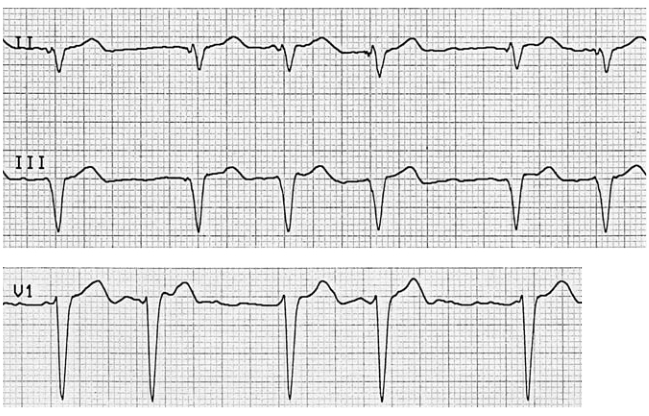
\includegraphics[width=0.80\textwidth]{./Bilder/VHFEKG_fein.png}
\caption[VHF im EKG]{Die Ableitungen II, III und V$_1$ eines Elektrokardiogramms. Zu sehen sind feine Flimmerwellen und eine absolute Kammerarrhythmie. Entnommen aus  \cite{gertsch_ekg_2007}.} 
\label{fig:EKG_afib}
\end{figure} 

%TODO Störungen im EKG? Ableitungsanzahl?